\chapter{O ciclo de vida do produto na I4.0}
\label{cha:ciclo-de-vida}
	
	Este capítulo visa trazer discussões sobre o impacto do amplo compartilhamento da memória digital do produto ao longo da cadeia de suprimentos por meio de serviços na Indústria 4.0.
	
	São abordadas possíveis mudanças na curva de ciclo de vida do produto e o surgimento de novos modelos de negócio baseado em dados (\textit{data-driven}).
	
	Uma visão da MDP sobre o eixo ``Ciclo de Vida e Cadeia de Valor'' do RAMI4.0 é abordada, discutindo melhor o porquê e as atribuições dos AASs como ``tipos'' e como ``instâncias''.
	

\section{Ciclo de vida do produto no RAMI4.0}
	
	O modelo do RAMI4.0 apresenta um eixo de ciclo de vida generalizado, derivado da norma IEC 62890 \cite{adolphs2015rami}. O objetivo deste eixo é representar o ciclo de vida de um Componente I4.0 ao longo de toda a sua cadeia de valor.
	
	Os ``tipos'' estão presentes desde a concepção/conceitualização até os primeiros protótipos/testes. O ``tipo'' de um ativo é definido pelas suas propriedades e funcionalidades distintas. Todos os itens que são criados ao longo do projeto de um produto (e.g., desenhos em CAD, manuais, \textit{softwares}, etc) são incorporados ao ``tipo'' do ativo. Informações externas associadas ao ativo que são criadas ao longo de seu desenvolvimento como informações de \textit{marketing} também são incorporadas ao ``tipo''.
	
	As instâncias são criadas/produzidas/fabricadas com base nas informações de um ``tipo'' de ativo. Informações específicas sobre produção, logística, qualidade e testes são associadas à ``instância'' de um ativo. Nesta fase, os dados de uso são coletados e associados para então poderem ser armazenados na MDP e compartilhados com outros parceiros ao longo da cadeia de suprimentos. 
	
	O histórico completo do ciclo de vida do produto está associados à combinação entre ``tipo'' e a ``instância'' de um determinado produto. Estes dados podem ser aproveitados de forma inteligente para a geração de valor, gerando assim novos modelos de negócio.
	
	Os relacionamentos entre ``tipos'' e ``instâncias'' são cíclicos e possibilitam a retroalimentação de informações. Para os ativos de um produto, por exemplo, informações sobre seu uso e manutenção armazenadas na MDP podem auxiliar em melhorias no seu próprio processo de fabricação, além de ser fonte de dados para o desenvolvimento de novas versões aperfeiçoadas do mesmo produto, gerando um novo ``tipo''.
	
	Portanto, esse fluxo de informações entre ambas as fases de um produto são essenciais para a melhoria de seu próprio projeto. A \autoref{fig:aas-lifecycle} ilustra como ocorre a instanciação (criação de uma instância a partir de um tipo) e o uso da MDP das ``instâncias'' para a criação de novas versões de um ``tipo''.
	
	\begin{figure}[htb!]
		\centering
		\caption{Ciclo de vida do produto.}
		\label{fig:aas-lifecycle}
		\includegraphics[width=1\textwidth]{aas-lifecycle}
		\fonte{O autor.}
	\end{figure}

\section{Extração de informações pela MDP na fase ``tipo''}

	A extração de informações da MDP do produto auxilia no desenvolvimento de versões de ``tipos'' aprimoradas.

	Com os ciclos de vida do produto cada vez mais curtos e cadeias de logística cada vez mais complexas, explorar o registro informações do produto pode garantir uma posição competitiva de uma empresa comercial frente aos competidores.
	
	Além disso, a memória digital do produto abre novas possibilidades em relação ao combate à pirataria e falsificação de produtos, na proteção ao consumidor e na garantia de qualidade do produto \cite{wahlster2007digitalmemory}.
	
	A análise de dados da MDP possibilita o aprimoramento do ``tipo'' do produto das seguintes maneiras:
	
	\begin{itemize}
		\item Identificação e reparo de falhas de projeto;
		\item Adição de novas funcionalidades ao produto;
		\item Melhoria da experiência do cliente/operador com o produto;
		\item Geração de indicadores de sustentabilidade.
	\end{itemize}

	A \autoref{tab:produto-tipo} exemplifica possíveis informações e seus respectivos submodelos que agregam valor ao produto por meio da geração de novos ``tipos''.
	
	\begin{table}[htb]
		\centering
		\caption{Possíveis informações e respectivos submodelos para o aprimoramento do projeto do produto.}
		\label{tab:produto-tipo}
		\begin{tabular}{p{4cm}p{3cm}p{3cm}p{4cm}}
			
			\hline
			\textbf{Informação}
			& \textbf{Submodelo}
			& \textbf{Cliente}
			& \textbf{Leitura}	
			\\ 
			
			\hline
			Histórico de leitura de sensores dos componentes
			& Leitura de sensores
			& Fabricante / Técnico de manutenção
			& Automática (E.g, a cada 6 horas)
			\\
			
			\hline
			Índice de disponibilidade, eficiência e qualidade do produto
			& Eficiência Global do Equipamento (OEE)
			& Fabricante / Gestor
			& Automática, sob solicitação
			\\
			
			\hline
			Volume de emissão de gases do efeito estufa
			& Pegada ambiental
			& Fabricante / Consumidor
			& Automática
			\\
			
			\hline
			Consumo energético
			& Eficiência energética
			& Fabricante / Consumidor / Operador
			& Automática, a cada turno
			\\
			
			\hline
			Funcionalidades mais utilizadas
			& Dados de uso
			& Fabricante
			& Automática
			\\
			
			\hline
			Leitura de coordenadas geográficas
			& Geolocalização
			& Gestor / Distribuidor / Consumidor
			& Sob solicitação
			\\

			\hline
		\end{tabular}
		\fonte{O autor.}
	\end{table}

	O \textbf{histórico de leitura de sensores dos componentes} permite ao fabricante monitorar remotamente determinados modelos de produtos por ele fabricados e identificar padrões de falha em determinadas peças.
	
	O monitoramento dos dados de sensores de temperatura, pressão, vibração e outros, atrelado a técnicas de análise de dados sobre um grande volume de dados (\textit{big data}) permite aos projetistas identificar erros estruturais de projeto do produto e com isso realizar a reparação e lançamento como um novo ``tipo''.
	
	A frequência de escrita das informações na MDP pelo produto pode ser configurada pelo fabricante e a frequência de leitura também pode ser estabelecida pelo cliente que consome as informações.
	
	Os \textbf{índices de disponibilidade, eficiência e qualidade} do produto permitem a realização do cálculo de eficiência global do equipamento (Overall Equipment Effectivences - OEE). O OEE demonstra se uma máquina está funcionando perfeitamente ou se necessita de algum reparo, caso haja a queda do índice médio.
	
	Caso o OEE de diversos clientes apontem uma eficiência abaixo do esperado, o fabricante é capaz de investigar o problema e eventualmente reprojetar o equipamento. Além disso, o próprio gestor da área pode monitorar o índice de eficiência de seus equipamentos
	
	O \textbf{volume de emissão de gases do efeito estufa} pode identificar uma avaria no funcionamento do produto. Além disso, a alta emissão de gases pode ir contra as condições regulatórias do país e também oferecer riscos ao operador inserido no ambiente de trabalho.
	
	O monitoramento das emissões pode apontar a necessidade de mudança de projeto para atender às condições legais e de saúde do trabalhador.
	
	O \textbf{consumo energético} acima ou abaixo dos padrões estabelecidos em projeto também pode indicar um funcionamento incorreto ou abaixo de sua capacidade. A análise do consumo e eventuais correções em projeto são necessárias para fornecer ao consumidor uma melhor qualidade em operação.
	
	As informações de \textbf{funcionalidades mais utilizadas} podem ser utilizadas pelo fabricante para a determinação de funções do produto que podem não ser claras para o consumidor ou funções que estão sendo utilizadas da maneira errada.
	
	Mudanças na ergonomia do produto, remoções de funcionalidades raramente utilizadas e melhorias na intuitividade das funções de operação são mudanças de projeto que elevam a experiência do operador/consumidor com o produto e causam uma maior percepção de valor.


\section{Extração de informações pela MDP na fase ``instância''}

	A fase ``instância'' ocorre com a produção e venda de um produto com base nas informações de um ``tipo'' de ativo \cite{bader2019aas}. As informações específicas sobre produção, logística e qualidade são associadas às ``instâncias'' dos ativos.
	
	Nesta fase o produto está em produção, o que significa que consumidor/operador está ativamente utilizando o equipamento em sua empresa. Os dados de uso da instância podem ser compartilhados com outros parceiros da cadeia de valor.
	
	A análise de dados da MDP traz benefícios às ``instâncias'' sem necessariamente alterar seu projeto (alterar seu tipo). Alguns benefícios são elencados a seguir:	

	\begin{itemize}
		\item Manutenção do produto orientada por dados
		\item Eficiência logística e simplificação da logística reversa (reciclagem, acionamento da garantia, \textit{recalls}, etc)
		\item Maior interação com as partes da cadeia de suprimentos
	\end{itemize}

	\begin{table}[htb]
		\centering
		\caption{Possíveis informações e respectivos submodelos extraídos de ``instâncias'' de produtos.}
		\label{tab:produto-instancia}
		\begin{tabular}{p{4cm}p{3cm}p{3cm}p{4cm}}
			
			\hline
			\textbf{Informação}
			& \textbf{Submodelo}
			& \textbf{Cliente}
			& \textbf{Leitura}	
			\\
			
			\hline
			Histórico de leitura de sensores dos componentes
			& Leitura de sensores
			& Fabricante / Técnico de manutenção
			& Automática
			\\
			
			\hline
			Leitura de coordenadas geográficas
			& Geolocalização
			& Gestor / Distribuidor / Consumidor
			& Sob solicitação
			\\
			
			\hline
			Manuais, notas fiscais, certificados de manutenção
			& Documentação
			& Gestor / Consumidor / Fabricante (escrita)
			& Sob solicitação
			\\

			\hline
		\end{tabular}
		\fonte{O autor.}
	\end{table}

	O histórico de leitura de sensores dos componentes permite não somente a indicação de pontos de melhoria de projeto, mas também uma mudança de paradigma em relação à forma como a manutenção dos equipamentos é realizada.
	
	Com o histórico de leitura de sensores de cada componente do equipamento, estratégias de manutenção de ativos preditivas e prescritivas podem ser adotadas pelo próprio fabricante. A manutenção orientada por dados de uso pode reduzir a incidência de falhas e trazer benefícios econômicos \cite{odonovan2015maintenance}.
	
	Com a manutenção prescritiva, os dados empíricos e o histórico do ativo são utilizados para prescrever qual medida deve ser tomada, trazendo mais confiabilidade por meio de técnicas estatísticas. A contínua extração de dados de sensores da MDP e sua análise torna a ação de manutenção mais automatizada.
	
	As \textbf{leituras de coordenadas geográficas} são úteis durante o transporte de produtos entre os membros da cadeia de suprimentos. O distribuidor, por exemplo, pode ter acesso à posição exata do produto enquanto este estiver sob sua custódia.
	
	As coordenadas geográficas garantem a rastreabilidade do produto enquanto ele se desloca ao longo da cadeia de suprimentos. A demanda de rastreabilidade surge para manter um melhor controle da cadeia produtiva, assim como repassar essas informações aos consumidores.
	
	O submodelo de documentação contém todos os documentos digitais referentes ao produto. \textbf{Manuais, notas fiscais, certificados de manutenção} e outros documentos podem ser escritos, lidos e atualizados pelos parceiros da CS mediante autenticação.
	
	O compartilhamento de documentos digitais permite uma maior interação com as partes e garante que cada um terá sempre a versão mais atualizada de um determinado documento, assim como favorece a gestão de documentos, reduzindo o uso do papel e tornando os ambientes de trabalho mais seguros, ágeis e organizados.
	
	Os documentos representam uma conexão entre os membros da CS, portanto, comunicados, formulários de troca de produto, documentos para acionamento de garantia do produto, \textit{recalls} e quaisquer outras operações que envolvam a logística reversa podem ser solicitados pela própria MDP.